\section{Preliminary phases}
The first set of experiments was partially implemented parallel to model development. This choice allowed us to fully understand each part of the model, and to identify and correct some important errors, not discussed in the previous section. Since the beginning, the main project requirement was to work in limit conditions for the system, in order to analyse each result with respect to the worst case, and determine a lower bound for the system performance. \\

% --- Optical bench
The first thing to do, was to build an optical bench. After many attempts, we made a solid support in which we could fix a laser-camera pair, that allowed us to:
  \begin{itemize}
    \item change the distance between the laser and the camera;
    \item change the triangulation angle, defined as the angle between the optical axis of the camera and the baseline;
    \item change the tilt angle of the lens (only with respect to the $y$ axis)
  \end{itemize}
This first setup was made using a couple of aluminum extrusion profiles, rigidly connected to each other, and a protractor to correctly evaluate the angle of the camera. We used a special case for the camera, that allowed us to set the lens tilt, shielding the sensor from the external light. Furthermore, the case lets to add an interferential filter between the lens and the sensor, cutting all unwanted light frequencies. The laser projection defines a plane parallel to the ground, while the camera looks it from the upside. The accuracy in the distance measurement between the various elements is $1 \, mm$ for the linear distances, and $1 \, degree$ for the angles. The characteristics of the camera and of the laser are shown in Table \ref{tab:conf1}.
  \begin{table}[h!]
  \centering

  \begin{tabular}{ccccc}
    \hline
    \multicolumn{5}{|c|}{\textbf{Camera}}                                                                                                                                                                            \\ \hline
    \multicolumn{1}{|c|}{\textbf{Name}} & \multicolumn{1}{c|}{\textbf{Size}}      & \multicolumn{1}{c|}{\textbf{Pixel size}} & \multicolumn{1}{c|}{\textbf{Lens Manufacturer}} & \multicolumn{1}{c|}{\textbf{Focal}} \\ \hline
    \multicolumn{1}{|l|}{}              & \multicolumn{1}{c|}{\textit{pix x pix}} & \multicolumn{1}{c|}{\textit{$\mu$m}}        & \multicolumn{1}{c|}{}                           & \multicolumn{1}{c|}{\textit{mm}}    \\ \hline
    \multicolumn{1}{|l|}{Spectra}       & \multicolumn{1}{c|}{1710 x 1690}        & \multicolumn{1}{c|}{8.0}                 & \multicolumn{1}{c|}{Linos}                      & \multicolumn{1}{c|}{25}             \\ \hline
    \multicolumn{1}{l}{}                & \multicolumn{1}{l}{}                    & \multicolumn{1}{l}{}                     & \multicolumn{1}{l}{}                            & \multicolumn{1}{l}{}                \\ \cline{2-4}
    \multicolumn{1}{c|}{}               & \multicolumn{1}{c|}{\textbf{Laser}}     & \multicolumn{1}{c|}{}                    & \multicolumn{1}{c|}{}                           &                                     \\ \cline{2-4}
    \multicolumn{1}{c|}{}               & \multicolumn{1}{c|}{\textbf{Frequency}} & \multicolumn{1}{c|}{\textbf{Power}}      & \multicolumn{1}{c|}{\textbf{Aperture}}          &                                     \\ \cline{2-4}
    \multicolumn{1}{c|}{\textit{}}      & \multicolumn{1}{c|}{\textit{nm}}        & \multicolumn{1}{c|}{\textit{W}}          & \multicolumn{1}{c|}{\textit{degree}}            & \textit{}                           \\ \cline{2-4}
    \multicolumn{1}{c|}{}               & \multicolumn{1}{c|}{660}                & \multicolumn{1}{c|}{0.05}                & \multicolumn{1}{c|}{45}                         &                                     \\ \cline{2-4}
  \end{tabular}
  
  \caption{Configuration of the first system.}
  \label{tab:conf1}
\end{table}

% --- The code
\noindent
The second element we needed, was the software. To perform out test, we realized a simple library, written in \textsc{MatLab} \cite{MATLAB:2017}, that implements a calibration algorithm for \acs{SOL} systems, a way to extract the laser from the acquired images, all subpixel filters, described in Section \ref{sec:laser-peaks}, and some scripts to perform our evaluation. Many of these functions were implemented using the \textsc{Image Processing Toolbox}, but many others were implemented from scratch, in order to deeply analyse each operation. The choice to use \textsc{MatLab} was taken for its speed of prototyping and for the type of mathematical operations we are interested in. \\

% --- Calibration process
Once the bench and the software were ready, we had to calibrate the system, and the algorithm we used was Tsai, described in \cite{TsaiTvLenses}. As we  just said, Tsai takes in input a grid of points, both in sensor and in world reference systems, to perform the calibration. To get these points, we tried to use a 2D checkerboard, placed in a plane consistent with the one of the laser. Our idea was to compare the results of Tsai with those of the calibration algorithm in \textsc{MatLab}. So we used two different checkerboards, one with squares size of $9 \, mm$ (shown in Figure \ref{fig:calib1}) and one with squares size of $29 \, mm$. \\
Unfortunately this approach could not work. First of all, the \textsc{Image Processing Toolbox} needed at least two images of the checkerboard, taken in different positions, but it was impossible for us because of the bond on checkerboard position in the laser plane. Furthermore, we observed that, despite our attention in building the system, the laser plane was not completely parallel to the ground one, that means that the checkerboard didn't lie on the same plane of the laser. This introduced another problem: even if we had used Tsai, calibration points would not have met the reality, and our measures will be lost their meanings. Thus, we understood we needed to extend our model, adding laser compensations described with Equations \ref{eq:radial-compensations}, before converting points from the world to the camera. \\

To solve this problem, we decided to use a 3D reference object, of which we know all dimensions, but this type of calibration is pretty different from the previous one. To build the grid of points for Tsai we have to move the target along all the \acs{FOV} of the camera, and to process each acquired frame in order to determine some points of interests. Hence, the target is mounted on a very precise step motor that we move with known steps. In Figure \ref{fig:calib2} we shown a live acquisition of the target: as we can see it is not perpendicular to the optical axis of the camera, that sees something like the one shown in Figure \ref{fig:calib3}. A simple technique to make the grid that we are interested in, is to locate the corner of the holes, as we shown in Figure \ref{fig:calib4}. To detect these points, we need both the frontal and internal profile of the hole: the points will be the intersection of the two line. If we don't have these two information, the diffraction due to laser engraving on the edge of the hole added to many noise to identify the point correctly. Then, if the target was perpendicular to the camera, the inner side wasn't visible. \\
  \begin{figure}[t!]
    \centering
    \begin{minipage}[c]{.48\textwidth}
      \centering
      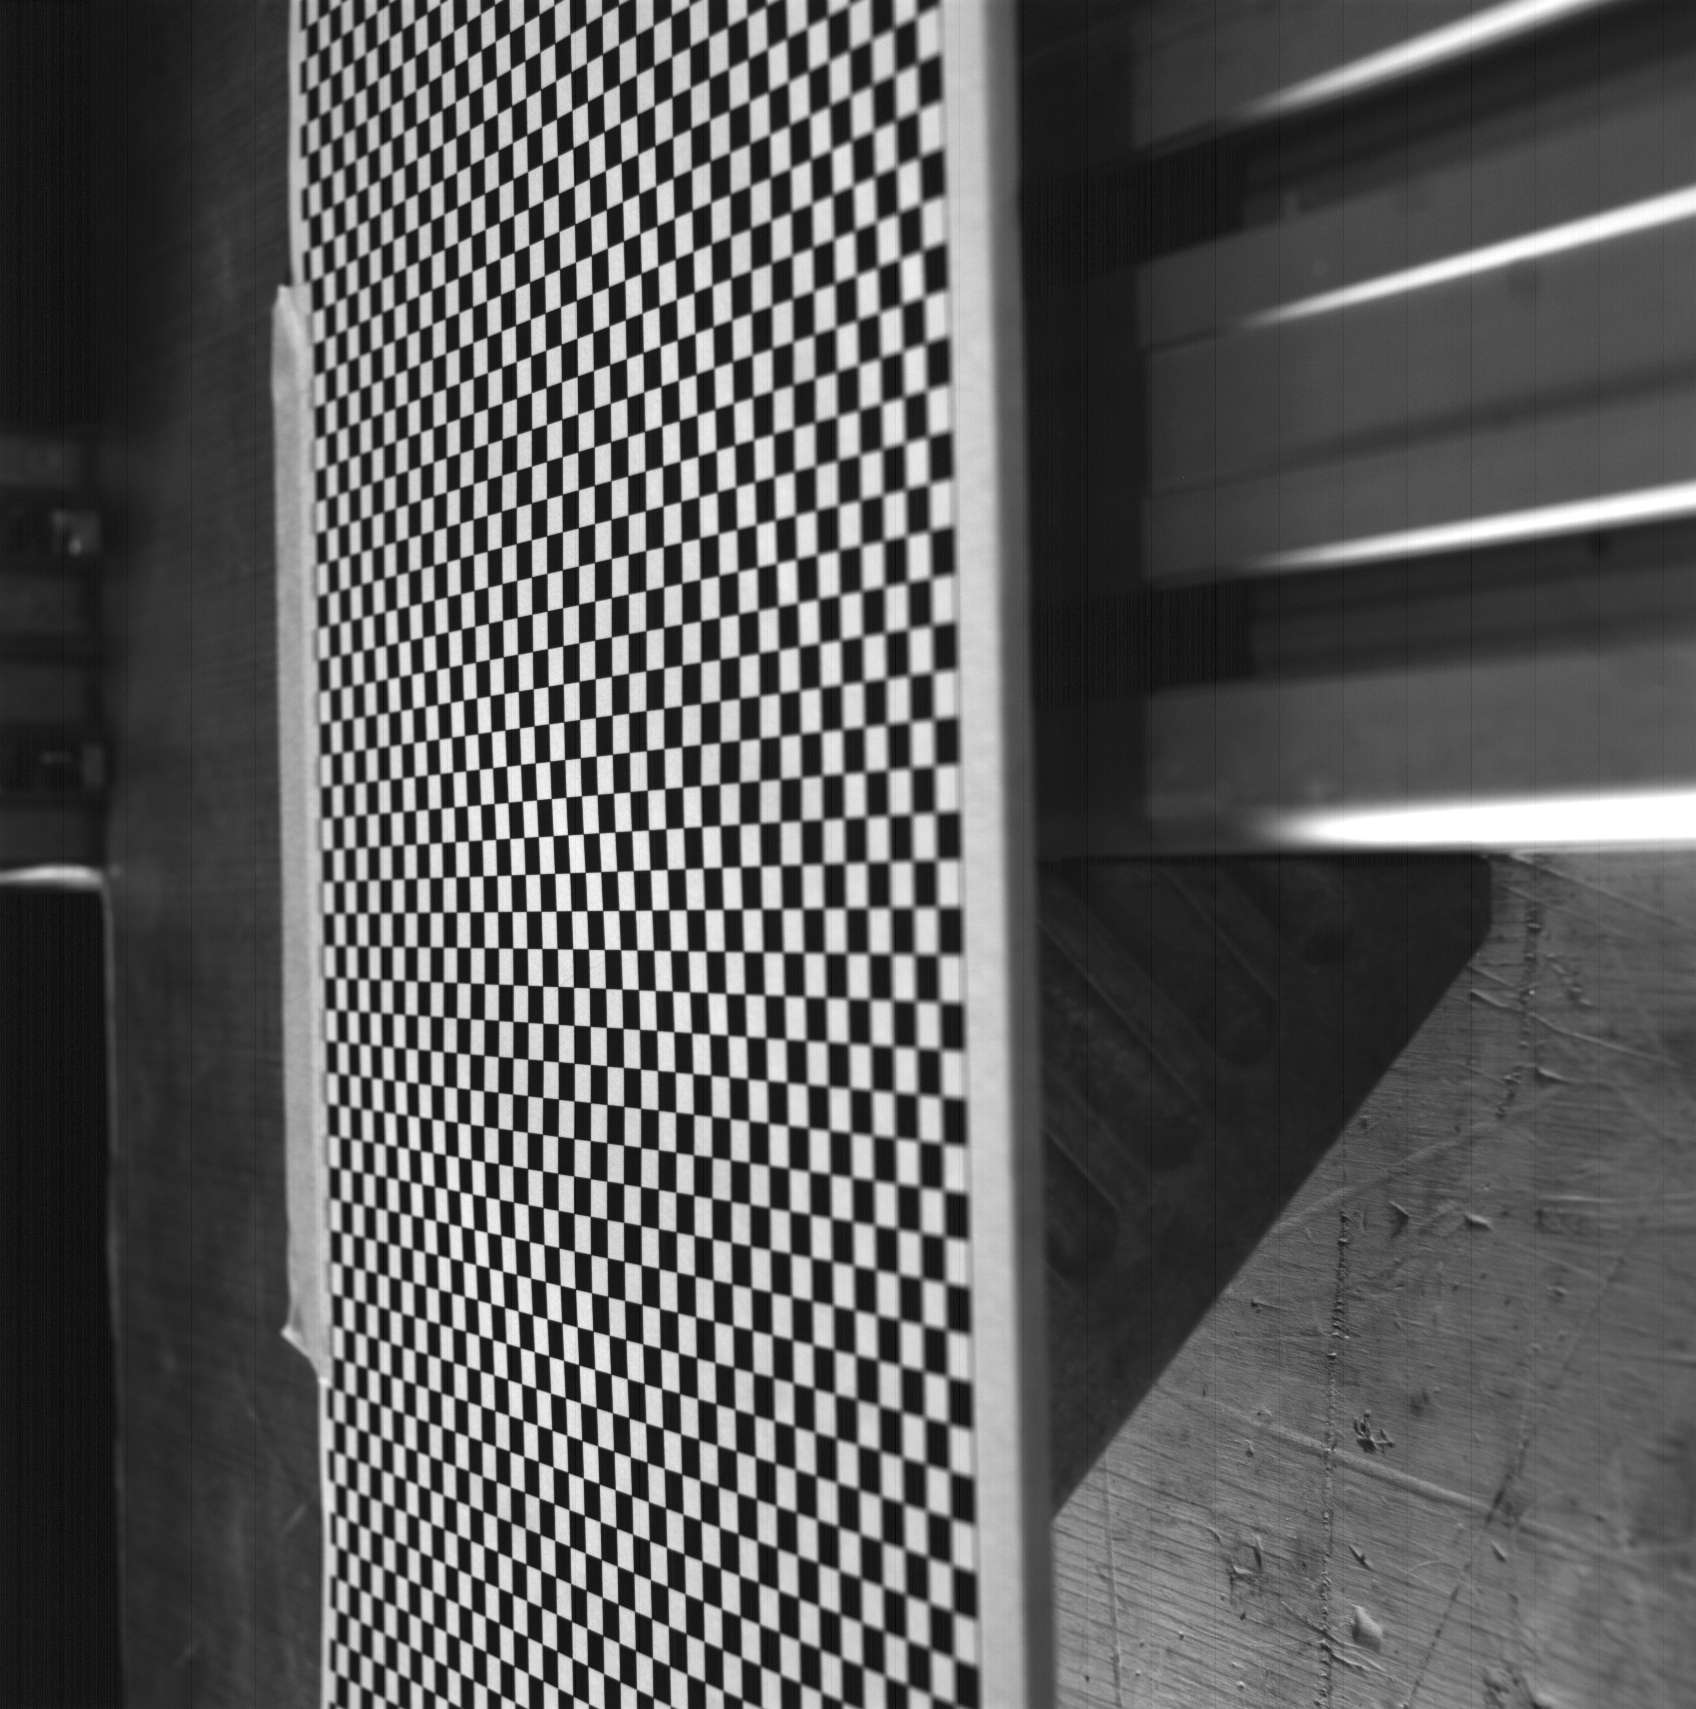
\includegraphics[angle=270, origin=c, width=\textwidth]{./images/analysis/checker09.jpg}
      \caption{Calibration checker with size of squares of $9 \, mm$.}
      \label{fig:calib1}
    \end{minipage}
    \hfill
    \begin{minipage}[c]{.48\textwidth}
      \centering
      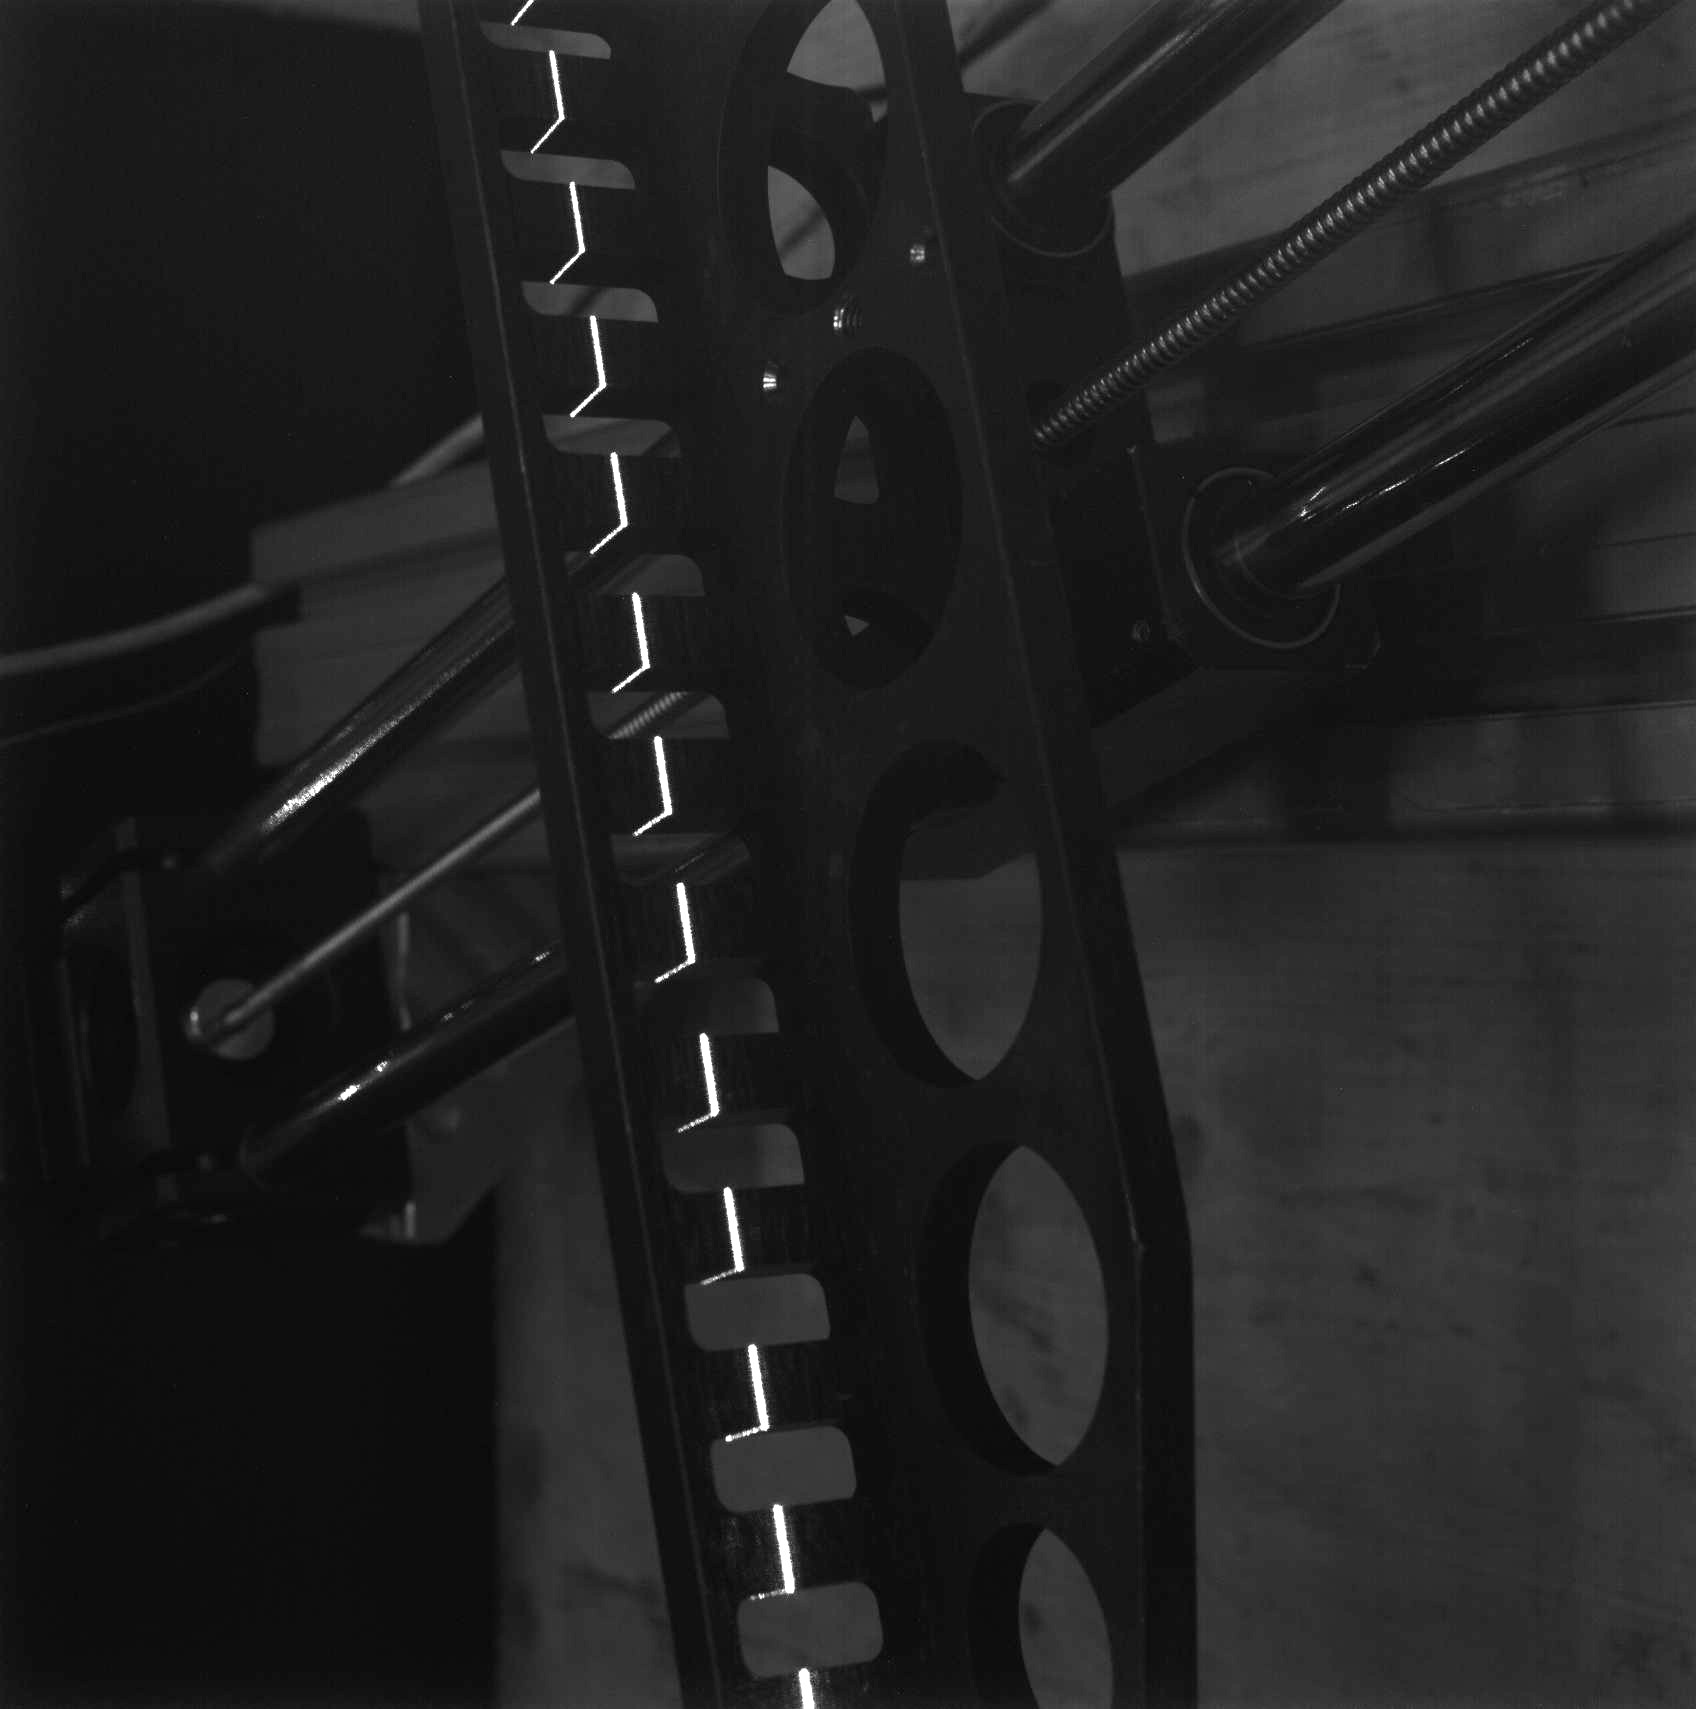
\includegraphics[angle=270, origin=c, width=\textwidth]{./images/analysis/gage.jpg}
      \caption{3D calibration target. \\ ~}
      \label{fig:calib2}
    \end{minipage}
  \end{figure}

  \begin{figure}[t!]
    \begin{minipage}[c]{.48\textwidth}
      \centering
      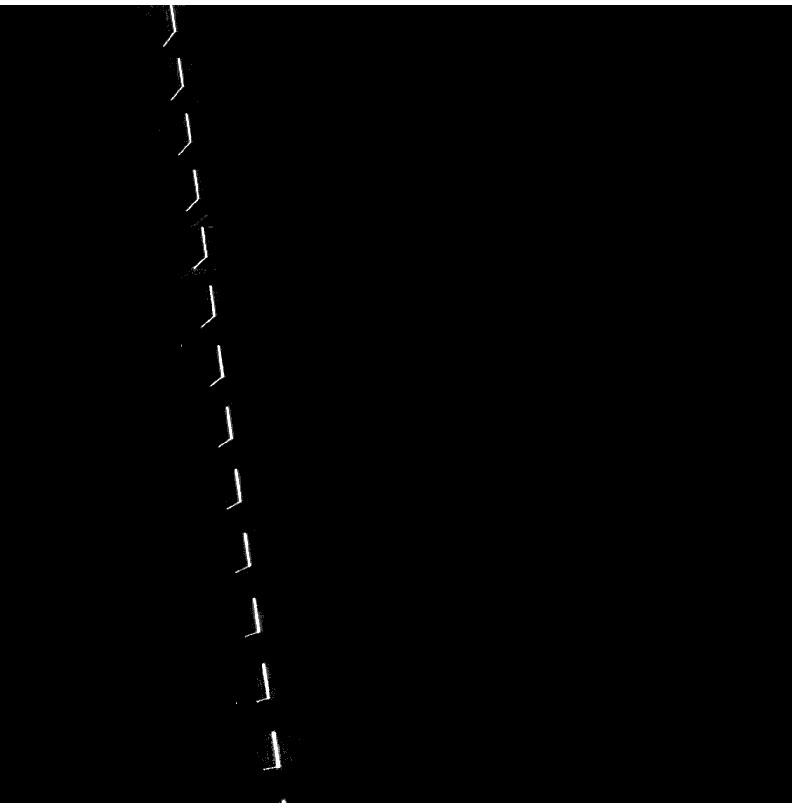
\includegraphics[angle=270, origin=c, width=\textwidth]{./images/analysis/laser_profile_over-gage.jpg}
      \caption{Target profile acquired by the camera.}
      \label{fig:calib3}
    \end{minipage}
    \hfill
    \begin{minipage}[c]{.48\textwidth}
      \centering
      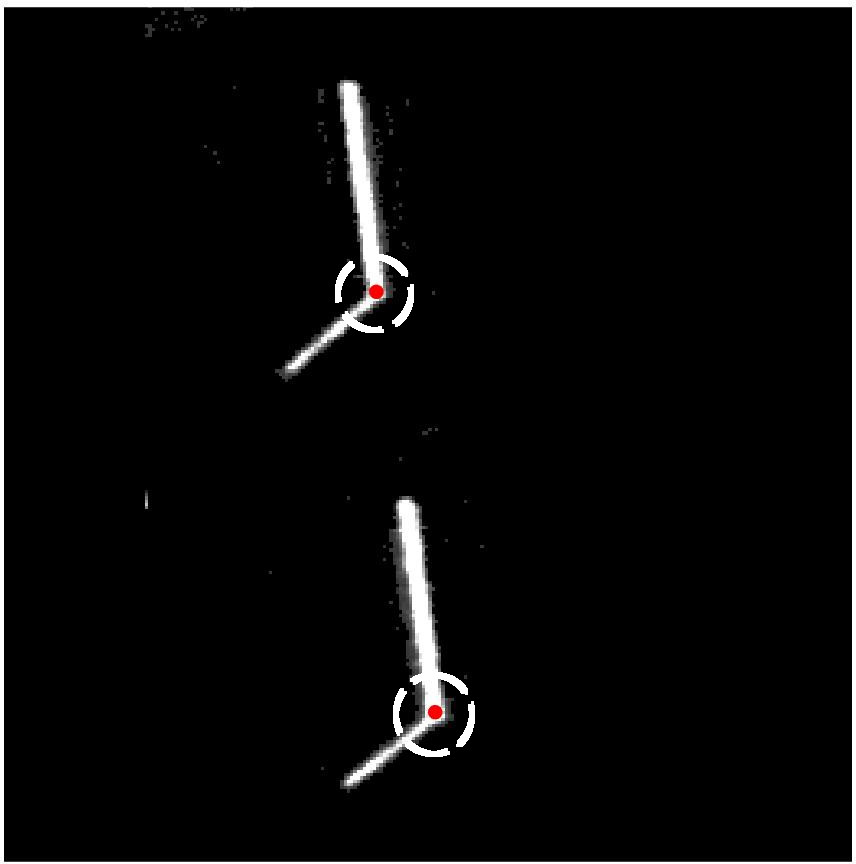
\includegraphics[angle=270, origin=c, width=\textwidth]{./images/analysis/laser_profile_over-gage_corner_det.jpg}
      \caption{Keypoint needed fot the calibration phase.}
      \label{fig:calib4}
    \end{minipage}
  \end{figure}
%    \vfill
%    \begin{minipage}[c]{.48\textwidth}
%      \centering
%      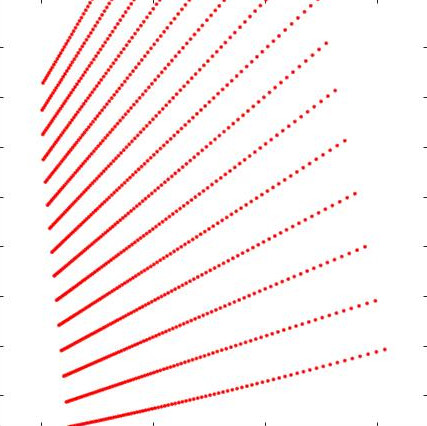
\includegraphics[angle=180, origin=c, width=0.7\textwidth]{./images/analysis/grid.jpg}
%      \caption{Final grid}
%      \label{fig:calib5}
%    \end{minipage}
%    \hfill
%    \begin{minipage}[c]{.48\textwidth}
%      \centering
%      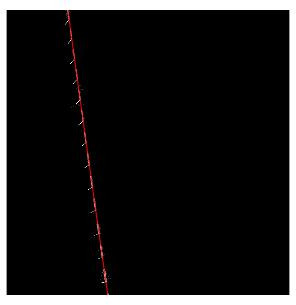
\includegraphics[angle=270, origin=c, width=0.7\textwidth]{./images/analysis/laser_profile_over-gage_fitted.jpg}
%      \caption{Keypoint needed fot the calibration phase.}
%      \label{fig:calib6}
%    \end{minipage}

In the process just described, it is important to consider radial distortion of the lens. What we see in Figure \ref{fig:calib3} is not a straight line, as it is in reality, but because of radial distortion it is a parabola. This mistake leads to the construction of a completely erroneous grid. Another effect of target rotation with respect to the optical axis, is the orientation of the world reference system. This is not a problem, but it is used to apply a correction in order to align the $y$ axis with the \acs{FOV} of the camera, as we assumed in Figure \ref{fig:laser-triang-pdv}. \\

\begin{table}[!t]
  \centering
  \begin{tabular}{@{}cccc@{}}
    \toprule
    \textbf{Measure} & \textbf{Our version}                                                     & \textbf{\textsc{Company version}}                                          & \textbf{Unit}  \\
    \midrule
    $f$ & $36.542$                                                      & $31.971$                                                      & $\left[mm\right]$ \\ && \\
    $k_1$ & $2.24 \cdot 10^{-5}$                                      & $2.3 \cdot 10^{-5}$                                         & $\left[\frac{1}{mm^2}\right]$ \\&& \\
    $T$ & $\begin{bmatrix} 161.605 \\ -35.215 \\ -465.005 \end{bmatrix}$ & $\begin{bmatrix} -157.381 \\ -26.830 \\ 407.198 \end{bmatrix}$ & $\left[mm\right]$ \\&& \\
    $R$ & $\begin{bmatrix}
        -0.770 & -0.638 &  0.015 \\
        -0.415 &  0.482 & -0.772 \\
         0.485 & -0.600 & -0.636 \\
      \end{bmatrix}$ & $\begin{bmatrix}
	     0.765 &  0.644 &  0.009 \\
	     0.480 & -0.562 & -0.673 \\
	    -0.429 &  0.519 & -0.739 \\
      \end{bmatrix}$ & ~ \\ && \\
    $s_x$ & $1$ & $1$ & ~ \\ && \\
    $\left( C_x, C_y \right)$ & $\left(512, 512\right)$                 & $\left(484.387, 918.144\right)$        & $\left[pix\right]$ \\
    \bottomrule
  \end{tabular}
  
  \caption{Comparison between two different version of Tsai's algorithm}
  \label{tab:calib-comparison}
\end{table}
	
In Table \ref{tab:calib-comparison} we compared the results of our implementation of Tsai, with results of a precise implementation, used in industrial systems. The parameters we are interested in are the intrinsic ones. As we can see, the main difference is done by the principal point: in fact, our implementation does not take into account this optimization, so it assumes that the principal point is located in the image center. This is pretty true along the $x$ axis, but not enough along $y$, accordingly with the other version. Furthermore, the difference in focal length is due to the lack of precision of the \textsc{MatLab} optimization functions. \\
As far as extrinsic parameters, however, they depend on the choice of the world reference system that is arbitrarily, thus the sign differences are negligible. From this quick analysis we can concluded not only that our implementation is precise enough for our purposes, but also that the results that we will reach will be a slack lower bounds, that could be improved in real systems implementations. \\
